
\chapter{Traducci\'on de requerimientos PDDL} \label{pagcap5}
	
	En el cap\'itulo \ref{pagcap2} analizamos el lenguaje STRIPS. 
        Este formalismo describe acciones en
        t\'erminos de precondiciones y efectos. Las precondiciones 
        de las acciones son conjunciones de literales positivos, al igual que los
        estados inicial y final. Los efectos de las acciones son
        expresados como una conjunci\'on de literales. Esta
        definici\'on de STRIPS,
        m\'as el predicado de igualdad y su negaci\'on, conforman el
        lenguaje de representaci\'on soportado por el Planificador
        Continuo presentado en el cap\'itulo \ref{pagcap3}. Luego, 
        estudiamos el lenguaje PDDL e identificamos los
        siguientes requerimientos que est\'an siendo considerados para el
        desarrollo del presente trabajo: igualdad, efectos
        condicionales, precondiciones disyuntivas y precondiciones universales.

        En este cap\'itulo vamos a identificar y definir variantes
        para STRIPS. Tales variantes surjen adicionando los
        requerimientos anteriores a la especificaci\'on de dicho lenguaje. 
        Adem\'as, estableceremos una notaci\'on
        equivalente en PDDL para estas variantes y analizaremos la
        teor\'ia subyacente. Por \'ultimo, propondremos formas de
        procesar cada variante para una posterior implementaci\'on en
        el traductor propuesto.
	
	La organizaci\'on del presente cap\'itulo es la siguiente. 
        En la secci\'on \ref{cap5:inicial} se define un marco
        te\'orico incluyendo resultados preliminares, las nociones
	de {\bf esquemas de compilaci\'on} y {\bf compilabilidad} y 
        algunos supuestos de simplificaci\'on. En las secciones subsiguientes 
        se discute, de manera te\'orica, la traducci\'on de cada una
	de las variantes STRIPS identificadas. 
        En la secci\'on \ref{cap5:strips} se muestra la traducci\'on \emph{trivial} para
	STRIPS est\'andar. Posteriormente, en la
        secci\'on \ref{cap5:pddll}, se analiza STRIPS con literales
        negativos y el predicado de igualdad. A este formalismo lo
        denotaremos PDDL$_{L}$. En la secci\'on \ref{cap5:efectoscond}
	se analiza STRIPS con efectos condicionales, 
        STRIPS$_{\emph{C}}$ y su equivalente PDDL$_{\emph{C}}$. La
        secci\'on \ref{cap5:preconddisy} presenta STRIPS con precondiciones disjuntivas, 
	STRIPS$_{D}$ y PDDL$_{D}$. 
        En la secci\'on \ref{cap5:precondUniv} se introduce
	uno de los resultados m\'as importantes de nuestra
	investigaci\'on. Este resultado formaliza y demuestra una nueva variante
	de STRIPS que incluye precondiciones cuantificadas
	universalmente. Tal variante es llamada
        STRIPS$_{\emph{u}}$ con su equivalente PDDL$_{\emph{u}}$.
        Por \'ultimo, todos los ejemplos en este cap\'itulo concluyen con la representaci\'on
        STRIPS para cada dominio traducido. Tal representaci\'on
        es similar a la definida para el Planificador Continuo.
	
	
\section{Marco Te\'orico} \label{cap5:inicial}

	
	Existe un \emph{trade-off}\footnote{Un balance aceptable entre 
	dos cosas opuestas con el fin de lograr un objetivo.} entre la 
	expresividad y la ``gesti\'on''\footnote{En Ingl\'es, \emph{manageability}.} 
	de un lenguaje formal de definici\'on de dominios de planificaci\'on.
	Un lenguaje pr\'actico deber\'ia tener un nivel lo m\'as alto posible 
	para poder representar problemas de una manera natural, exacta y simple. 
	Sin embargo, mientras m\'as se incrementa la complejidad de lenguaje en cuesti\'on, 
	m\'as se incrementa la dificultad para resolver el problema
	por parte de los planificadores. 
        En \cite{gbraun:Gazen97combiningthe}, Gazen y Knoblock, definen dos enfoques posibles 
	que permiten considerar un lenguaje m\'as expresivo de representaci\'on de dominios. 
	El primero, enuncia que para soportar un lenguaje m\'as
	expresivo se debe extender el algoritmo de planificaci\'on. 
	Mientras que el segundo enfoque, implica desarrollar un
	preprocesador que traduzca un dominio representado en un
	lenguaje m\'as expresivo a uno m\'as simple. 
	Si bien, esta \'ultima propuesta no podr\'ia manejar 
        constructores m\'as expresivos de manera tan eficiente, 
        es m\'as simple desde el punto de vista conceptual. 
	Consideramos esta segunda propuesta para desarrollar el
	presente trabajo.

        Esta secci\'on presenta resultados y definiciones,
        introducidas por Nebel en \cite{gbraun:Nebel2000onthe} y \cite{gbraun:Nebel:2001:EPP}, 
        y adaptadas a las necesidades de nuestra
        implementaci\'on.
	

        \subsection{Esquemas de Compilaci\'on}
	
	En primer lugar, introducimos la
        definici\'on de instancia de planificaci\'on para luego continuar el estudio
        sobre los esquemas de compilaci\'on.

	%%%%%% Instancia de planificacion

        \begin{definition}

        Sea $\Sigma$ un conjunto finito de \texttt{\'atomos
        proposicionales}, $O$ un conjunto finito de operadores y
        $\hat{\Sigma} = \top \cup \bot \cup literales(\Sigma)$ donde,
        $\top$ denota \texttt{verdadero}, $\bot$ denota
        \texttt{falso} y $literales(\Sigma)$ es el conjunto de
        literales definidos sobre $\Sigma$.

	Una {\bf instancia de planificaci\'on} es una 
	tupla $\Pi = \left\langle \Xi,I,G \right\rangle$ donde:
	
	\begin{itemize}
	
	\item $\Xi = \left\langle \Sigma,O \right\rangle $ es una estructura 
	de dominio que consiste de un conjunto finito de \'atomos proposicionales 
	y un conjunto finito de operadores,
	
	\item $I \subseteq \Sigma $ es el estado inicial, y
	
	\item $G \subseteq \hat{\Sigma} $ es la especificaci\'on de la meta.
	
	\end{itemize}
	
	\end{definition}

        La estructura $\Xi$ es el dominio de planificaci\'on compuesto
        por acciones (tambi\'en llamadas operadores en la
        bibliograf\'ia) mientras que los conjuntos $I$ y $G$ 
        conforman la especificaci\'on del problema de planificaci\'on.
        
        A continuaci\'on, damos una noci\'on intuitiva del
        concepto de esquemas de compilaci\'on y, posteriormente,
        presentamos este concepto de manera formal, adaptando la
        definici\'on propuesta por Nebel.

        Un formalismo de planificaci\'on $X$ es tan expresivo como otro 
	formalismo $Y$ si, los dominios de planificaci\'on y los planes formulados 
	en $Y$, son expresables en $X$ de manera
	concisa. B\'asicamente, un esquema de compilaci\'on es 
	una soluci\'on que preserva el mapeo entre las estructuras de
	dominio en el formalismo $X$ y en el formalismo $Y$. La
        siguiente definici\'on expresa este concepto.
	
	\begin{definition}
	
	Un {\bf esquema de compilaci\'on\footnote{En Ingl\'es, \emph{compilation
	scheme}.}} de $X$ a $Y$ es una tupla de funciones 
	$f = \left\langle f_{\xi},f_{i},f_{g} \right\rangle $ que inducen una funci\'on $F$
	de instancias de $X$, $\Pi = \left\langle \Xi,I,G \right\rangle $, a instancias de $Y$,
	$F(\Pi)$, como sigue:
	
	\begin{center}
		
	$F(\Pi) = \left\langle f_{\xi}(\Xi),I \cup f_{i}(\Xi),G \cup f_{g}(\Xi) \right\rangle $
	
	\end{center}
		
	y satisfacen las siguientes condiciones:
		
	\begin{itemize}
		
	\item existe un plan para $\Pi$, si y s\'olo si, existe un plan
          para $F(\Pi)$, y
		
	\item el tama\~{n}o de los resultados de $f_{\xi},f_{i}$ y $f_{g}$ es 
	polinomial en el tama\~{n}o de los argumentos.
		
	\end{itemize}
	
	\end{definition}

        Si bien, esta definici\'on establece condiciones referidas a la complejidad
        computacional de las funciones $f_{\xi},f_{i}$ y $f_{g}$, esto no
        es un factor limitante en nuestra investigaci\'on. Sin embargo,
        en el caso general, procuramos definir esquemas de compilaci\'on
        eficientes en t\'erminos de complejidad computacional. 

        En este sentido, establecemos los siguientes supuestos relacionados
        a este tipo de mapeos:

        \begin{enumerate}

        \item No haremos ninguna restricci\'on sobre los recursos
        computacionales, por lo tanto, un
	an\'alisis exhaustivo de la complejidad computacional queda
	fuera del alcance del presente trabajo.

        \item Las estructuras de dominio son traducidas de manera
        independiente respecto de la descripci\'on del estado
        inicial y la meta del problema de planificaci\'on.

        \item No existe ninguna restricci\'on sobre el tama\~{n}o
        de los dominios involucrados en el mapeo.

        \item La longitud del plan resultante es preservada en
        \emph{cierto grado}. Este supuesto ser\'a retomado m\'as adelante
        cuando expliquemos compilabilidad.
        
        \end{enumerate}


        En la siguiente secci\'on analizaremos y definiremos
        formalmente la noci\'on de compilabilidad.


        \subsection{Compilabilidad}

        A partir de los conceptos que aparecen en \cite{gbraun:Nebel:2001:EPP}, vamos a
        enunciar una definici\'on relacionada al tama\~{n}o de los planes.
	
	\begin{definition}
	
	Sea \texttt{f} un esquema de compilaci\'on, $\Delta$ un
	plan que resuelve la instancia de planificaci\'on $\Pi$ y $\Delta^{'}$ un plan que
	resuelve la instancia de planificaci\'on $F(\Pi)$. Mediante 
	$||\Delta||$ denotamos el tama\~{n}o de un plan para el
	formalismo fuente y mediante $||\Delta^{'}||$ denotamos el tama\~{n}o de
	un plan para el formalismo destino.
	Asimismo, mediante $||\Pi||$ se denota el tama\~{n}o de la instancia.
	
        Entonces:
	
	\begin{itemize}
	
	\item \texttt{f} es un {\bf esquema de compilaci\'on que preserva exactamente el tama\~{n}o del plan}
	si $||\Delta^{'}|| \leq ||\Delta|| + k $, para alguna
	constante entera positiva $k$. 
	
	\item \texttt{f} es un {\bf esquema de compilaci\'on que preserva linealmente el tama\~{n}o del plan}
	si $||\Delta^{'}|| \leq c x ||\Delta|| + k $, para las
	constantes positivas $c$ y $k$.
	
	\item \texttt{f} es un {\bf esquema de compilaci\'on que preserva polinomialmente el tama\~{n}o del plan}
	si $||\Delta^{'}|| \leq p(||\Delta||, ||\Pi||) $, para alg\'un
	polinomio $p$.
	
	\end{itemize}
	\end{definition}
	
        A continuaci\'on, formalizamos la relaci\'on de
        compilabilidad\footnote{En Ingl\'es, \emph{compilability}.}.
	
	\begin{definition}
	
	Un formalismo de planificaci\'on $X$ es {\bf compilable} al formalismo 
	$Y$, expresado como $X \preccurlyeq^{x} Y$, si y s\'olo si,
	existe un esquema de compilaci\'on de $X$ a $Y$.
	
	Entonces:
	
	\begin{itemize}
	
	\item Si $X \preccurlyeq^{1} Y$, entonces el tama\~{n}o del plan es preservado exactamente.
	
	\item Si $X \preccurlyeq^{c} Y$, entonces el tama\~{n}o del plan es preservado 
	linealmente (en $||\Delta||$).
	
	\item Si $X \preccurlyeq^{p} Y$, entonces el tama\~{n}o del plan es preservado 
	polinomialmente (en $||\Delta||$ y $||\Pi||$).
	
	\item Si $X \preccurlyeq^{x}_{p} Y$, entonces la compilaci\'on
        es en tiempo polinomial y el tama\~{n}o del plan es preservado 
	polinomialmente (en $||\Delta||$ y $||\Pi||$).
	
	\end{itemize}
	
	\end{definition}
	
	Los casos en los que la compilaci\'on de formalismos 
	preserva el tama\~{n}o de un plan, ya sea exacta o linealmente,
	indican que el formalismo destino que estamos considerando 
	es, al menos, tan expresivo como el formalismo fuente.
	Sin embargo, si un esquema de compilaci\'on requiere 
	de un crecimiento polinomial respecto al tama\~{n}o de los planes,
	entonces el formalismo fuente es m\'as expresivo que 
	el formalismo destino.
	
	Por \'ultimo, en \cite{gbraun:Nebel:2001:EPP}, se enuncian dos propiedades importantes
	para la relaci\'on de com\-pi\-la\-bi\-li\-dad:
	

	\begin{proposition} \label{cap5:reflex} 
	
	Las relaciones $\preccurlyeq^{x}$ y $\preccurlyeq^{x}_{p}$ 
	son reflexivas y transitivas.
	
	\end{proposition}
	
	\begin{proposition}  
	
	Si $X \sqsubseteq Y$, entonces $X \preccurlyeq^{1}_{p} Y$.
	
	\end{proposition}
	

	
	
	%%%%%%%%%%%%%%%%%%%%%%%%%%%%%%%%%%%%%%%%%%%%%%%%%
	

	
        En las siguientes secciones clasificaremos y ejemplificaremos 
        las variantes STRIPS con\-si\-de\-ra\-das y propondremos una
        notaci\'on equivalente para PDDL. Adem\'as, usando la
        relaci\'on de compilabilidad, definiremos esquemas de
        compilaci\'on que luego ser\'an implementados en nuestro
        traductor. Para esto, proponemos las capas de
        traducci\'on que se indican en la figura \ref{gbraun:layers}.


        \begin{figure}[h!]
	\centering
		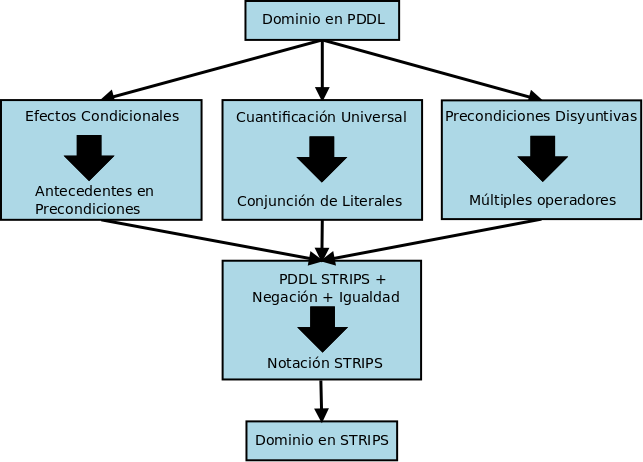
\includegraphics[width=10cm,height=9cm]{capastrad.png}
		\caption{Capas de Traducci\'on}
		\label{gbraun:layers}
	\end{figure}


%	\section{STRIPS y STRIPS$_{L}$} \label{cap5:stripsigualdad}

        \section{PDDL$_{STRIPS}$} \label{cap5:strips}


        El STRIPS est\'andar, estudiado en el cap\'itulo \ref{pagcap2} y
        definido por Russell y Norving en \cite{gbraun:Rus09},
        es el formalismo m\'as b\'asico de esta
        clasificaci\'on en t\'erminos de expresividad. B\'asicamente,
        describe acciones mediante precondiciones y efectos.
        Las precondiciones son conjunciones de literales positivos al
        igual que los estados inicial y final. Los efectos son
        expresados como una conjunci\'on de literales. Los literales positivos
        son inclu\'idos en la lista de agregados y los negativos en la
        lista de borrados de la acci\'on. STRIPS est\'andar no permite
        efectos condicionales, disyunci\'on ni cuantificaci\'on
        universal en precondiciones.

        A continuaci\'on, estudiaremos la traducci\'on de STRIPS
        expresado en PDDL.
	

        \begin{proposition} \label{cap5:trivial}
	$STRIPS \preccurlyeq^{1} STRIPS$.
        \end{proposition}

        \begin{proof}
        Por propiedad reflexiva de la relaci\'on de compilabilidad,
        proposici\'on \ref{cap5:reflex}, concluimos que STRIPS
        es \emph{compilable} a STRIPS preservando exactamente el
        tama\~{n}o de los planes. 
        \end{proof}

        Luego, si denotamos como PDDL$_{STRIPS}$ al formalismo PDDL
        acotado a la expresividad de STRIPS y lo reemplazamos 
        en la proposici\'on anterior, podemos concluir que:

        \begin{corolario} \label{cap5:trivial}
	$PDDL_{STRIPS} \preccurlyeq^{1} STRIPS$
        \end{corolario}
        
        Por lo tanto, PDDL$_{STRIPS}$ es \emph{compilable} a
        STRIPS est\'andar preservando exactamente el tama\~{n}o de
        los planes. Este lenguaje es el m\'as b\'asico en t\'erminos de
        expresividad.

        Veamos, mediante un ejemplo, c\'omo
        PDDL$_{STRIPS}$ es traducido a STRIPS. 

        \begin{ejemplo}

        Dada una instancia del problema del ``Mundo de Bloques'' en
        PDDL$_{STRIPS}$, la traducci\'on procede adicionando efectos
        negados a la lista de borrados y efectos positivos a la lista
        de agregados de la especificaci\'on STRIPS.

        \begin{verbatim}
% Dominio PDDL
(define (domain bkw)
(:requirements :strips)
(:predicates (clear ?x)
             (ontable ?x)
             (armempty)
             (holding ?x)
             (on ?x ?y))

(:action pickup
  :parameters (?ob)
  :precondition (and (clear ?ob) (armempty))
  :effect (and (holding ?ob) (not (clear ?ob)) (not (armempty))))

(:action stack
  :parameters  (?ob ?underob)
  :precondition (and  (clear ?underob) (holding ?ob))
  :effect (and (clear ?ob) (on ?ob ?underob) (armempty)
               (not (clear ?underob)) (not (holding ?ob))))
)

% Problema PDDL
(define (problem pb1)
   (:domain bkw)
   (:objects a b c)
   (:goal (on a b))
   (:init (ontable c) (ontable b) 
          (on a c) (clear a) (clear b) (armempty))
)
        \end{verbatim}
        La representaci\'on en STRIPS del problema anterior es la
        siguiente:
        \begin{verbatim}

% pickup(X,Y)
Precondiciones: clear(X), armempty
Borrados: clear(X), armempty
Agregados: holding(X)

% stack(X,Y)
Precondiciones: clear(Y), holding(X)
Borrados: clear(Y), holding(X)
Agregados: armempty, clear(X), on(X,Y)


% Problema STRIPS
holds(ontable(c),init)
holds(ontable(b),init)
holds(on(a,c),init)
holds(clear(a),init)
holds(clear(b),init)
holds(armempty,init)
        \end{verbatim}
        \end{ejemplo} 

        En base a lo expuesto, podemos concluir que PDDL$_{STRIPS}$ es soportado por el
        Planificador Continuo.



%	\subsection{STRIPS$_{L}$}

        \section{PDDL$_{L}$} \label{cap5:pddll}

        En el caso del predicado de igualdad, el escenario que se presenta es
        diferente. STRIPS est\'andar no soporta el uso de este
        predicado en las precondiciones, no obstante, es aceptado
        en algunas variantes STRIPS. 
        Ocurre algo similar para el caso de la negaci\'on ya que no est\'a incluida en
        la definici\'on de STRIPS. Algunos planificadores aceptan
        negaci\'on pero, \'unicamente, del predicado igualdad. Este es el caso del lenguaje de 
        representaci\'on del Planificador Continuo.          

        Por su parte, PDDL si permite incluir negaci\'on en las precondiciones
        y en las metas de los
        problemas de planificaci\'on posibilitando la definici\'on de
        acciones como indicamos a continuaci\'on:

        \begin{ejemplo}%{Negaci\'on de literales en precondiciones}
        
        Podemos modelar en PDDL la acci\'on \textt{stack} del 
        ``Mundo de Bloques'' permitiendo que un bloque, \textt{?X}, sea apilado 
        sobre otro, \textt{?Z}, si \textt{?Z} no es un bloque.

        \begin{verbatim}
(:action stack
   :parameters (?X ?Y ?Z)
   :precondition (and (clear ?X) (clear ?Z) (on ?X ?Y) (not (block ?Z)))
   :effects (and (on ?X ?Z) (clear ?Y) (not (on ?X ?Y))) 
)
        \end{verbatim}
        \end{ejemplo}

        Sin embargo, como mencionamos al
        inicio de esta secci\'on, esta caracter\'istica no es
        soportada directamente por STRIPS est\'andar, por lo tanto, es
        necesaria una traducci\'on. 

        La adici\'on de la negaci\'on a STRIPS da lugar a otra variante
        del formalismo llamada STRIPS$_{L}$. Esta variante tiene la
        particularidad, a diferencia de STRIPS
        est\'andar, de permitir negaci\'on de literales en las
        precondiciones. 

        A continuaci\'on, enunciamos, sin
        demostrar, el siguiente resultado postulado por Nebel 
        en \cite{gbraun:Nebel2000onthe}:


        \begin{proposition} \label{cap5:stripsLtostrips}
        $STRIPS_{L} \preccurlyeq^{1}_{p} STRIPS$
        \end{proposition}

        A partir de este resultado, concluimos que STRIPS$_{L}$ es
        \emph{compilable} a STRIPS, en tiempo
        polinomial y el tama\~{n}o de los planes es
        preservado exactamente. 
        
        En este sentido, tambi\'en definimos a PDDL$_{L}$ como el formalismo obtenido de restringir
        PDDL al requerimiento de negaci\'on (STRIPS
        est\'a impl\'icito por ser el requerimiento por defecto de
        PDDL). Dado que PDDL$_{L}$ es lo mismo que
        STRIPS$_{L}$ en t\'erminos de nivel expresivo y, por  
        la proposici\'on \ref{cap5:stripsLtostrips}, podemos concluir que:

        \begin{corolario} 
        $PDDL_{L} \preccurlyeq^{1}_{p} STRIPS$
        \end{corolario}

        Es decir, PDDL$_{L}$ es \emph{compilable} a STRIPS en tiempo
        polinomial y el tama\~{n}o de los planes es
        preservado exactamente. 

        La definici\'on original de STRIPS$_{L}$ enunciada por Nebel
        s\'olo establece el uso de
        literales negativos en precondiciones, pero nada concluye
        sobre la aceptaci\'on, o no, del predicado de igualdad. Adem\'as, la
        igualdad no es soportada por STRIPS est\'andar, aunque s\'i es
        soportada por el lenguaje de representaci\'on del
        Planificador Continuo.

        Entonces, con el objetivo de incluir el predicado en el contexto de un
        subconjunto acotado de PDDL, en este trabajo de tesis, vamos a considerar
        el predicado de igualdad como parte de STRIPS$_{L}$ y, en
        consecuencia, de PDDL$_{L}$

        El pr\'oximo ejemplo muestra c\'omo modelar acciones
        en PDDL$_{L}$ usando el predicado de igualdad:

        \begin{ejemplo}%{Igualdad en PDDL}

        La acci\'on \texttt{stack}
        permite apilar un bloque s\'olo si el destino es 
        la mesa. \texttt{table} es una constante.

	\begin{verbatim}
(:action stack
   :parameters (?X ?Y)
   :precondition (and (clear table) (= ?Y table)) 
   :effect (and (on ?X table) (not (clear table)))
)                
	\end{verbatim}
	\end{ejemplo}
  
        Por \'ultimo, es necesario definir una restricci\'on
        importante sobre PDDL$_{L}$ para que pueda ser \'integramente
        soportado por el Planificador Continuo. 
        Dicha restricci\'on es impuesta sobre el requerimiento
        de negaci\'on:

        \begin{itemize}

        \item Permitiremos el uso del \texttt{not}, en precondiciones, s\'olo cuando
        es aplicado junto con el pre\-di\-ca\-do de igualdad, tal es el caso
        del t\'ermino \texttt{(not (= ?Y ?Z))}\footnote{Existen otras
        alternativas para tratar con la negaci\'on en precondiciones
        como la presentada por Gazen y
        Knoblock \cite{gbraun:Gazen97combiningthe} para el
        planificador Graphplan. Sin embargo, un an\'alisis exhaustivo
        de estas alternativas est\'a fuera del alcance de esta investigaci\'on.}.

        \end{itemize}

        Veamos, mediante un ejemplo, c\'omo traducir PDDL$_{L}$ a la
        representaci\'on STRIPS del Pla\-ni\-fi\-ca\-dor Continuo.

        \begin{ejemplo}
        
        Traducimos la siguiente acci\'on con el predicado de igualdad
	a notaci\'on STRIPS:

	\begin{verbatim}
(:action stack
   :parameters (?X ?Y)
   :precondition (and (clear table) (= ?Y table)) 
   :effect (and (on ?X table) (not (clear table)))
)                
	\end{verbatim}

        \begin{verbatim}
% stack(X,Y)
Precondiciones: clear(table), Y == table
Borrados: clear(table)
Agregados: on(X,table)             
	\end{verbatim}

        Y la negaci\'on del predicado de igualdad en precondiciones:

	\begin{verbatim}
(:action stack
   :parameters (?X ?Y)
   :precondition (and (clear ?Y) (not (= ?Y table))) 
   :effect (and (on ?X ?Y) (not (clear ?Y)))
)                
	\end{verbatim}

        es traducido como:

        \begin{verbatim}
% stack(X,Y)
Precondiciones: clear(Y), Y \== table
Borrados: clear(Y)
Agregados: on(X,Y)             
	\end{verbatim}
        \end{ejemplo}

        A partir de lo expuesto, podemos concluir que PDDL$_{L}$, con la restricci\'on impuesta sobre
        el predicado PDDL de igualdad y la negaci\'on, es
        soportado por el Planificador Continuo.
	

%%%%%%% EFECTOS CONDICIONALES
	
%	\section{STRIPS$_{\emph{C},L}$} \label{cap5:efectoscond}

        \section{PDDL$_{\emph{C}}$} \label{cap5:efectoscond}

        El formalismo obtenido de adicionar {\bf efectos condicionales} a
        STRIPS es llamado STRIPS$_{\emph{C}}$. 
        Gazen y Knoblock \cite{gbraun:Gazen97combiningthe} proponen una
        manera particular de tratar con estos efectos postulando el
        siguiente resultado, tambi\'en estudiado por Nebel en \cite{gbraun:Nebel:2001:EPP}:

        \begin{proposition}\label{gbraun:NebelEfectos}
		
	$STRIPS_{\emph{C}} \preccurlyeq^{x}_{p} STRIPS_{L} $
	
	\end{proposition} 
 
        El esquema propuesto por Gazen y Knoblock, tambi\'en formulado
        por Weld en \cite{gbraun:Weld99recentadvances}, es denominado
        {\bf expansi\'on total}\footnote{En Ingl\'es, \emph{full expansion}.}. Este
        enfoque es el m\'as simple\footnote{Weld \cite{gbraun:Weld99recentadvances}
        tambi\'en propone dos enfoques m\'as para realizar esta
        traducci\'on: Expansi\'on Factorizada, \emph{factored
        expansion} y Expansi\'on Parcialmente
        Factorizada, \emph{partially factored}. Ambos est�n fuera del
        alcance de la investigaci\'on.}. Como indica la
        figura \ref{gbraun:compiEF}, a partir de una acci\'on con efectos 
        condicionales, se generan esquemas de acciones STRIPS
        considerando todas las combinaciones consistentes de los
        antecedentes en los efectos condicionales. Esta alternativa
        tiene como ventaja la simplicidad, sin embargo, puede generar
        una cantidad exponencial de esquemas, a pesar de que no es
        com\'un a menos que se definan en conjunto con efectos cuantificados
        universalmente\footnote{Notar que la cuantificaci\'on
        universal en efectos no es soportada por nuestro traductor y
        est\'a fuera del alcance de la investigaci\'on. Por lo tanto,
        esta es una simplificaci\'on resultante de la definici\'on
        inicial del subconjunto PDDL establecido en el cap\'itulo \ref{pagcap2}.}.
	Si una acci\'on tiene $n$ efectos condicionales y cada uno contiene $m$ 
	conjuntos de antecedentes, la expansi\'on completa de una acci\'on puede producir
	$n^m$ acciones STRIPS. Este esquema de traducci\'on es tambi\'en analizado por Nebel 
        en \cite{gbraun:Nebel:2001:EPP} donde concluye que esta 
        traducci\'on no puede ser mejorada a\'un si se aceptan planes 
        que preservan su tama\~{n}o linealmente. 


        \begin{figure}[h!]
	\centering
		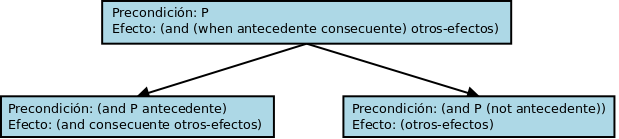
\includegraphics[width=14cm,height=3.5cm]{ef.png}
		\caption{Expansi\'on Total para Efectos Condicionales}
		\label{gbraun:compiEF}
	\end{figure}


        En este sentido, enunciamos la siguiente proposici\'on, asumiendo por
        simplificaci\'on, que aceptamos planes que preservan su
        tama\~{n}o polinomialmente.

	\begin{proposition}\label{propCLtoS}
		
	$STRIPS_{\emph{C}} \preccurlyeq^{x}_{p} STRIPS $
	
	\end{proposition} 

        \begin{proof}
        Aplicando la proposici\'on \ref{gbraun:NebelEfectos} y luego, por
        propiedad transitiva de la relaci\'on de compilabilidad,
        concluimos que $STRIPS_{\emph{C}} \preccurlyeq^{x}_{p} STRIPS $.
        \end{proof}

        Definiendo PDDL$_{\emph{C}}$ como una variante de PDDL
        con, \'unicamente, efectos condicionales y, dado que es lo
        mismo que STRIPS$_{\emph{C}}$ en t\'erminos de expresividad,
        reemplazamos en la proposici\'on anterior y obtenemos:

        \begin{corolario}
		
	$PDDL_{\emph{C}} \preccurlyeq^{x}_{p} STRIPS $
	
	\end{corolario} 

        De este resultado, concluimos que PDDL$_{\emph{C}}$ es
        \emph{compilable} a STRIPS en tiempo
        polinomial y el tama\~{n}o de los planes es
        preservado polinomialmente. 

        A continuaci\'on, vemos un ejemplo para analizar el esquema
        de traducci\'on definido en esta secci\'on y luego conclu\'imos
        sobre los supuestos de simplificaci\'on en relaci\'on al uso
        de efectos condicionales en acciones.
	 
	 \begin{ejemplo}
         
         Redefinimos la acci\'on \texttt{stack} del ``Mundo de
         Bloques'' en PDDL$_{\emph{C}}$, aplicamos 
         expansi\'on completa y mostramos los STRIPS
         equivalentes.

         \begin{verbatim}
(:action stack
   :parameters (?X ?Y ?Z)
   :precondition (and (clear ?X) (clear ?Z) (on ?X ?Y))
   :effects (and (on ?X ?Z) (clear ?Y) (not (on ?X ?Y)) 
                 (when (not (= table ?Z)) (not (clear ?Z))))
)
	\end{verbatim}

        Generamos las dos intancias de \texttt{stack} aplicando todas
        las combinaciones consistentes del antecedente del efecto condicional:

        \begin{verbatim}
(:action stack
   :parameters (?X ?Y ?Z)
   :precondition (and (clear ?X) (clear ?Z) 
                      (on ?X ?Y) (not (= table ?Z)))
   :effects (and (on ?X ?Z) (clear ?Y) 
                 (not (on ?X ?Y)) 
                 (not (clear ?Z)))
)

(:action stack1
   :parameters (?X ?Y ?Z)
   :precondition (and (clear ?X) (clear ?Z) 
                      (on ?X ?Y) (= table ?Z))
   :effects (and (on ?X ?Z) (clear ?Y) (not (on ?X ?Y)))
)
	\end{verbatim}
	 
         Finalmente, expresamos estas acciones usando notaci\'on
         STRIPS:

        \begin{verbatim}
% stack(X,Y,Z)
Precondiciones: clear(X), clear(Z), on(X,Y), Z \== table 
Borrados: on(X,Y), clear(Z)
Agregados: on(X,Z), clear(Y)

% stack1(X,Y,Z)
Precondiciones: clear(X), clear(Z), on(X,Y), Z == table 
Borrados: on(X,Y)
Agregados: on(X,Z), clear(Y)
	\end{verbatim}
	\end{ejemplo}
	
        A partir de este an\'alisis, establecemos los siguientes supuestos de
        simplificaci\'on para modelar dominios de planificaci\'on
        con efectos condicionales:

        \begin{enumerate}

        \item Los antecedentes s\'olo pueden ser de la forma: \texttt{(= X
        Y)} y \texttt{(not (= X Y))}. Esta restricci\'on se debe a que
        adem\'as de STRIPS est\'andar aceptamos el uso del predicado
        de igualdad y su negaci\'on en las precondiciones de las
        acciones.

        \item Los efectos condicionales pueden definir s\'olo un antecedente
        y s\'olo un consecuente.

        \end{enumerate}

        En base a lo expuesto, concluimos que PDDL$_{\emph{C}}$ es soportando por el
        Planificador Continuo con los supuestos establecidos previamente.

        
	 
%%%%%%%% PRECONDICIONES DISYUNTIVAS


%	\section{STRIPS$_{D}$} \label{cap5:preconddisy}

        \section{PDDL$_{D}$} \label{cap5:preconddisy}

        Las {\bf precondiciones disyuntivas} permite 
	el uso del operador \texttt{`or'} en precondiciones y
	descripciones de metas. Este operador no es soportando
        por STRIPS est\'andar y, por lo tanto, es necesario realizar un 
        prepocesamiento.

        A continuaci\'on, enunciamos y demostramos formalmente la
        relaci\'on entre STRIPS$_{D}$ y STRIPS.
	
	\begin{proposition}\label{propDtoS}
	
	$STRIPS_{D} \preccurlyeq^{1}_{p} STRIPS$
	
	\end{proposition}

        \begin{proof}
     
	En base a la proposici\'on $STRIPS_{D} \preccurlyeq^{1}_{p}
        STRIPS_{L}$, demostrada por Nebel
        en \cite{gbraun:Nebel:2001:EPP}, la proposici\'on \ref{cap5:stripsLtostrips}
	y la propiedad transitiva de la relaci\'on de compilabilidad, 
	conclu\'imos que existe un esquema de compilaci\'on de tiempo
        polinomial de $STRIPS_{D}$ a $STRIPS$ que preserva
        exactamente el tama\~{n}o del plan. El siguiente esquema de compilaci\'on ser\'ia una alternativa
        posible. 
        \ \\

        Sea $\Sigma$ un conjunto finito de \'atomos proposicionales y
        $L_{\Sigma}$ un conjunto de f\'ormulas conjuntivas compuestas por
        literales sobre $\Sigma$.
        Sea tambi\'en, $L$ un conjunto de literales y $L \subseteq \hat{\Sigma}$ donde
        $\hat{\Sigma} = \top \cup \bot \cup literales(\Sigma)$.

	Por cada operador:
        \begin{center}
	$o = \left\langle (c_{1} \vee ... \vee c_{n}),L \right\rangle$
        \end{center}

	donde $c_{i} \in L_{\Sigma}$, se generan los siguientes
        operadores:

        \begin{center}
	$o_{i} = \left\langle (c_{i}), L \right\rangle$ 
        \end{center}
        \end{proof}

        Dado que STRIPS$_{D}}$ es equivalente, en t\'erminos de
        expresividad, a PDDL con
        precondiciones disyuntivas como \'unico requerimiento, podemos
        denotar este formalismo como PDDL$_{D}$. Por lo tanto,
        concluimos el siguiente corolario:
	
        \begin{corolario}%\label{cap5:pddldstrips}
	
	$PDDL_{D} \preccurlyeq^{1}_{p} STRIPS$
	
	\end{corolario}

        Este corolario nos indica que PDDL$_{D}$ puede ser compilado a
        STRIPS en tiempo polinomial y preservando exactamente el
        tama\~{n}o de los planes.

	
        \begin{figure}[h!]
	\centering
		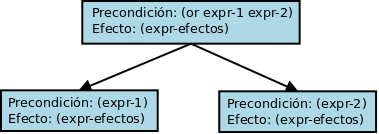
\includegraphics[width=8.5cm,height=3.5cm]{pd.png}
		\caption{Traducci\'on de Precondiciones Disyuntivas}
		\label{gbraun:predisytrad}
	\end{figure}

        Las precondiciones de las acciones que contienen disyunci\'on
	son expresadas en forma normal conjuntiva (i.e., como una
	conjunci\'on de disyunciones) y la compilaci\'on a STRIPS
	implica expresar esta precondici\'on como forma normal
	disyuntiva (i.e., como disyunci\'on de
	conjunciones). Por \'ultimo, cada subexpresi\'on de la
	disyunci\'on es la precondici\'on de una nueva acci\'on
	STRIPS como  muestra la figura \ref{gbraun:predisytrad}.
        A diferencia de los efectos condicionales, no hay un crecimiento
	exponencial de acciones dado que esta cantidad es 
        s\'olo proporcional a la cantidad de disyuntores
	en la precondicion de la acci\'on.

        El pr\'oximo ejemplo ilustra la traducci\'on propuesta:

        \begin{ejemplo}%{Traducci\'on de PDDL$_{D}$ a PDDL$_{STRIPS}$}

        La precondici\'on incluye el nuevo requerimiento \texttt{or} 
        estableciendo que un objeto, \texttt{?X}, puede ser apilado sobre
	un objeto, \texttt{?Z}, si \texttt{?Z} es la mesa (\texttt{istable}) u 
        otro bloque sin ning\'un bloque apilado.
	
	\begin{verbatim}		  
(:action stack
   :parameters (?X ?Y ?Z)
   :precondition (and (or (istable ?Z) (clear ?Z))
                      (clear ?X) (on ?X ?Y))
   :effect (and (on ?X ?Z) (clear ?Y)
                (not (clear ?Y)) (not (on ?X ?Y)))
)	
	\end{verbatim}

        Luego, la precondici\'on queda expresada de la siguiente manera:

        \begin{verbatim}		  
(:action stack
   :parameters (?X ?Y ?Z)
   :precondition (or (and (istable ?Z) (clear ?X) (on ?X ?Y))
                     (and (clear ?Z) (clear ?X) (on ?X ?Y)))
   :effect (and (on ?X ?Z) (clear ?Y)
                (not (clear ?Y)) (not (on ?X ?Y)))
)	
	\end{verbatim}
        
        El paso final del algoritmo consiste en generar una nueva
        acci\'on \texttt{stack1} con los mismos efectos que la
        acci\'on original.

        \begin{verbatim}		  
(:action stack
   :parameters (?X ?Y ?Z)
   :precondition (and (istable ?Z) (clear ?X) (on ?X ?Y))
   :effect (and (on ?X ?Z) (clear ?Y)
                (not (clear ?Y)) (not (on ?X ?Y)))
)	


(:action stack1
   :parameters (?X ?Y ?Z)
   :precondition (and (clear ?Z) (clear ?X) (on ?X ?Y))
   :effect (and (on ?X ?Z) (clear ?Y)
                (not (clear ?Y)) (not (on ?X ?Y)))
)
	\end{verbatim}

        Por \'ultimo, escribimos las acciones en notaci\'on STRIPS:

        \begin{verbatim}
% stack(X,Y,Z)
Precondiciones: istable(Z), clear(X), on(X,Y)
Borrados: clear(Y), on(X,Y)
Agregados: clear(Y), on(X,Z)		  

% stack1(X,Y,Z)
Precondiciones: clear(Z), clear(X), on(X,Y)
Borrados: clear(Y), on(X,Y)
Agregados: clear(Y), on(X,Z)		  
	\end{verbatim}
	\end{ejemplo}
	

        En base a este an\'alisis, concluimos que PDDL$_{D}$ puede ser
        traducido a STRIPS y, por lo tanto, es
        soportado por el Planificador Continuo.
	
	
%%%%%%%%% PRECONDICIONES UNIVERSALES
	

        \section{PDDL$_{\emph{u}}$} \label{cap5:precondUniv}

        Las {\bf precondiciones universales} implican el uso del
        cuantificador universal \texttt{`$\forall$'}, usualmente
        le\'ido como ``para todo''. 
        El uso de este cuantificador
        en precondiciones permite modelar acciones del mundo real como,
        por ejemplo, el comando \texttt{rmdir} de \emph{UNIX}, 
        que elimina un determinado directorio si \emph{todos} los archivos dentro
	de \'el fueron eliminados previamente.
	
        Las precondiciones universales no son soportadas en STRIPS
        est\'andar y, por lo tanto, es necesaria una traducci\'on de este
        requerimiento. El enfoque es simple. Los cuantificadores universales son 
        traducidos a una conjunci\'on de literales. Cada uno de esos literales se genera
	instanciando el par\'ametro cuantificado con cada uno
	de los objetos declarados en la definici\'on del problema de planificaci\'on.
	
	\begin{ejemplo}%{Expresiones cuantificadas universalmente}

	Sean los objetos: \texttt{block1} y \texttt{block2} y 
        supongamos la siguiente precondici\'on: \texttt{(forall (?a)
	(clear(?a)))}. Instanciando \texttt{?a} con los objetos 
	\texttt{block1} y \texttt{block2} obtenemos la precondici\'on
	equivalente: \texttt{(and (clear(block1)) (clear(block2)))}.
	
	\end{ejemplo}


        Antes de formalizar la traducci\'on de precondiciones
        universales, vamos a introducir la definici\'on de
        \emph{Base de Herbrand} extra\'ida
        de \cite{gbraun:Weld99recentadvances}:
	
%Herbrand base	
	\begin{definition} \label{def:herbrand}
	
	Sea $\Delta$ una sentencia de primer orden y libre de
        funciones. La \texttt{Base de Herbrand} $\Upsilon$
	es definida, recursivamente, de la siguiente manera:\\

		$\Upsilon (\Delta)  =  \Delta$, si $\Delta$  no
		contiene cuantificadores \\
		
		$\Upsilon (\forall_{t_{1}} x \Delta (x)) = \Upsilon
                (\Delta_{1}) \wedge ... \wedge \Upsilon (\Delta_{n})$
        \ \\

        donde $\Delta_{i}$ corresponde a cada posible interpretaci\'on
        de $\Delta(x)$ bajo el universo compuesto por los
        objetos de tipo $t_{1}$ del problema de planificaci\'on.

	\end{definition}

        Adem\'as, establecemos los siguientes supuestos de simplificaci\'on:

        \begin{enumerate}

        \item La cuantificaci\'on universal s\'olo es permitida en
        precondiciones\footnote{PDDL permite el uso de
        cuantificaci\'on universal tambi\'en en metas.}. 

        \item El mundo a modelar incluye un conjunto finito y
        est\'atico de objetos. Para el ejemplo del ``Mundo de Bloques'', la cantidad
        de \emph{bloques} debe ser finita y permanecer invariable mientras se
        planifica la soluci\'on.

        \item Todos los objetos involucrados deben ser del mismo
        tipo. Por lo tanto, no explicitamos el tipo $t_{1}$ de los objetos, tal como
        lo expresa la definici\'on \ref{def:herbrand}. 
        Continuando con el ejemplo del ``Mundo de Bloques'', los \'unicos
        objetos declarados deben ser \emph{bloques}. 

        \end{enumerate}
	
        En este sentido, estamos en condiciones de formular y
	demostrar el siguiente teorema. Sea STRIPS$_{\emph{u}}$, el formalismo
	resultante de adicionar precondiciones universales al STRIPS
	est\'andar. Entonces:

	
	\begin{teorema} \label{teorema:UP}
		
	$STRIPS_{\emph{u}} \preccurlyeq^{1}_{p} STRIPS$
	
	\end{teorema} 
	

	\begin{proof}
	Vamos a demostrar que existe una esquema de compilaci\'on de
	tiempo polinomial que preserva exactamente el tama\~{n}o de
	los planes. Por definici\'on de \emph{Base de Herbrand} y por
	los supuestos de simplificaci\'on, podemos definir el
	siguiente esquema de compilaci\'on.
        \ \\

        Sea $\Sigma$ un conjunto finito de \'atomos proposicionales y
        $L_{\Sigma}$ un conjunto de f\'ormulas conjuntivas compuestas por
        literales sobre $\Sigma$.
        Sea tambi\'en, $L$ un conjunto de literales y $L \subseteq \hat{\Sigma}$ donde
        $\hat{\Sigma} = \top \cup \bot \cup literales(\Sigma)$.
	
	Para cada operador:
	
	\begin{center}
	$o = \left\langle (\forall x_{i} (c_{j}(x_{i}))), L \right\rangle$
	\end{center}
	
	donde $c_{j}(x_{i})$ son predicados de aridad $n$ y
        $c_{j}(x_{i}) \in L_{\Sigma}$,	
	es posible generar un nuevo operador expresado como una
        conjunci\'on de literales:
	
	\begin{center}
	$o = \left\langle (c(x_{1}) \wedge ... \wedge c(x_{n})), L \right\rangle$ 
	\end{center}

        Por lo tanto, aplicando la proposici\'on
        \ref{cap5:stripsLtostrips} y luego la propiedad transitiva de
        la relaci\'on de compilabiliad, concluimos que $STRIPS_{\emph{u}} \preccurlyeq^{1}_{p} STRIPS$.
	\end{proof}

        Dado que STRIPS$_{\emph{u}}$ es equivalente, en t\'erminos de
        expresividad, a PDDL con
        precondiciones universales como \'unico requerimiento, podemos
        denotar este formalismo como PDDL$_{\emph{u}}$. Luego,
        enunciamos el siguiente corolario:

	\begin{corolario} %\label{teorema:UP}
		
	$PDDL_{\emph{u}} \preccurlyeq^{1}_{p} STRIPS$
	
	\end{corolario} 

        Este corolario nos indica que PDDL$_{\emph{u}}$
	puede ser compilado a STRIPS en tiempo polinomial y
	preservando exactamente la longitud de los planes. 
        \ \\

        Aplicamos este resultado al siguiente ejemplo:

        
        \begin{ejemplo}

        La precondici\'on para la acci\'on \texttt{stack} es que todo objeto
        en el problema debe estar sobre la mesa (\texttt{ontable})
        para que dos bloques puedan ser aplilados.
	
	Dado el siguiente problema PDDL y la
	acci\'on \texttt{stack} definida en PDDL$_{\emph{u}}$:
	
	\begin{verbatim}
(define (problem pb1)
   (:domain bkwup)
   (:objects a b c)
   (:goal (on a b))
   (:init (ontable c) (ontable b) (ontable a) 
          (on a c) (clear a)  (clear b) (armempty))
)

(:action stack
  :parameters  (?ob ?underob)
  :precondition (and (forall (?block) (ontable ?block))
                     (clear ?underob) (holding ?ob))
  :effect (and (clear ?ob) (on ?ob ?underob) (armempty)
               (not (clear ?underob)) (not (holding ?ob)))
)
	\end{verbatim}

        Aplicamos el esquema de compilaci\'on presentado y obtenemos
	la siguiente acci\'on:

	\begin{verbatim}	
(:action stack
   :parameters (?ob ?underob)
   :precondition (and (ontable a) (ontable b)(ontable c)
                      (clear ?underob)(holding ?ob)) 
   :effect (and (clear ?ob) (on ?ob ?underob) (armempty)
               (not (clear ?underob)) (not (holding ?ob)))
)
	\end{verbatim}

Finalmente, la representamos en notaci\'on STRIPS.

	\begin{verbatim}
% stack(X,Y)
Precondiciones: ontable(a), ontable(b), ontable(c), clear(Y), holding(X)
Borrados: clear(Y), holding(X)
Agregados: clear(X), on(X,Y), armempty
	\end{verbatim}
	\end{ejemplo}


	A partir de lo expuesto en esta secci\'on, podemos concluir
        que la variante PDDL$_{\emph{u}}$ es soportada por el Planificador Continuo.
        \ \\

        En este cap\'itulo hemos definido los esquemas de traducci\'on correspondientes
        para los re\-que\-ri\-mien\-tos PDDL incluidos en la
        investigaci\'on. Tales esquemas permiten traducir una
        especificaci\'on en un subconjunto de PDDL a una
        representaci\'on equivalente en la notaci\'on STRIPS soportada
        por el Planificador Continuo.

        En el pr\'oximo cap\'itulo estudiaremos la arquitectura
        propuesta para el traductor, formalizaremos el lenguaje fuente
        y destino y detallaremos aspectos
        principales de la implementaci\'on en Ciao Prolog.


